\documentclass[uplatex,dvipdfmx,a4paper,11pt]{jsarticle}

\usepackage{docmute}


% 数式
\usepackage{amsmath,amsthm,amssymb}
\usepackage{bm}
% 画像
\usepackage{graphicx}

\usepackage{multirow}
\usepackage{wrapfig}
\usepackage{ascmac}
\usepackage{xcolor}


\usepackage{makeidx}
\makeindex

\graphicspath{{../../_Figures//}{../../_Figures/Rheology/}}

\usepackage{qrcode}
\setlength\lineskiplimit{0pt}
\setlength\normallineskiplimit{0pt}

\usepackage{qexam}

\usepackage{titlesec}
\titleformat*{\section}{\Large\bfseries}
\titleformat*{\subsection}{\large\bfseries}
\titleformat*{\subsubsection}{\normalsize\bfseries}
\titleformat*{\paragraph}{\normalsize\bfseries}

% ページ設定
% \pagestyle{empty}
% 高さの設定
\setlength{\textheight}{\paperheight}   % ひとまず紙面を本文領域に
\setlength{\topmargin}{-5.4truemm}      % 上の余白を20mm(=1inch-5.4mm)に
\addtolength{\topmargin}{-\headheight}  % 
\addtolength{\topmargin}{-\headsep}     % ヘッダの分だけ本文領域を移動させる
\addtolength{\textheight}{-40truemm}    % 下の余白も20mmに%% 幅の設定
\setlength{\textwidth}{\paperwidth}     % ひとまず紙面を本文領域に
\setlength{\oddsidemargin}{-5.4truemm}  % 左の余白を20mm(=1inch-5.4mm)に
\setlength{\evensidemargin}{-5.4truemm} % 
\addtolength{\textwidth}{-40truemm}     % 右の余白も20mmに
% 図と本文との間
%\abovecaptionskip=-5pt
%\belowcaptionskip=-5pt
%
% 全体の行間調整
% \renewcommand{\baselinestretch}{1.0} 
% 図と表
%\renewcommand{\figurename}{Fig.}
%\renewcommand{\tablename}{Tab.}
%

% \makeatletter 
% \def\section{\@startsection {section}{1}{\z@}{1.5 ex plus 2ex minus -.2ex}{0.5 ex plus .2ex}{\large\bf}}
% \def\subsection{\@startsection{subsection}{2}{\z@}{0.2\Cvs \@plus.5\Cdp \@minus.2\Cdp}{0.1\Cvs \@plus.3\Cdp}{\reset@font\normalsize\bfseries}}
% \makeatother 

\usepackage[dvipdfmx,%
 bookmarks=true,%
 bookmarksnumbered=true,%
 colorlinks=false,%
 setpagesize=false,%
 pdftitle={数式に頼らない直感的理解による材料設計のためのレオロジー⼊⾨},%
 pdfauthor={佐々木裕},%
 pdfsubject={},%
 pdfkeywords={レオロジー; 材料設計; }]{hyperref}
\usepackage{pxjahyper}

\usepackage{plext}

\usepackage{niceframe} 
\usepackage{framed}
\newenvironment{longartdeco}{%
  \def\FrameCommand{\fboxsep=\FrameSep \artdecoframe}%
  \MakeFramed {\FrameRestore}}%
 {\endMakeFramed}
 
\usepackage{siunitx}

\newcommand{\rmd}{\mathrm{d}}

\usepackage[inline]{showlabels}

\begin{document}


\question{演習問題 1}
内容を振り返るために、以下に示した文章例の中から適切な記述のものを複数選んでください。
\begin{qlist}
	\qitem 「ニュートン流動」についての、正しい言葉はどれでしょうか?
		\begin{qlist2}
			\qitem せん断応力は、せん断速度に比例します。
			\qitem せん断応力はせん断速度には依存しなくて、一定値となります。
			\qitem 粘度が一定である場合、速く変形すれば、生じる応力は大きくなります。
			\qitem ニュートン流体では粘度が一定だから、せん断速度によらずにせん断応力も常に一定となります。
			\qitem ニュートン流体では、せん断速度が変化しても粘度は一定の値となります。
		\end{qlist2}
		\vspace{3mm}
        \begin{itembox}[l]{解答}
            正しい選択肢:(a), (c), (e)\\
            (解説)
			\begin{itemize}
				\item ニュートン流動では、せん断応力はせん断速度に比例して、その比例定数が粘度となります。
				\item 逆に言えば、粘度が一定となるような流動特性を示すものがニュートン流動です。
			\end{itemize}
        \end{itembox}
	\qitem 流動を表す、「水面に板を浮かべたモデル」についての、正しい言葉はどれでしょうか?
		\begin{qlist2}
			\qitem 液体は常に流動するので、板に接している部分でも流れが生じています。
			\qitem 「固体と接している液体は、その相対的な移動速度が同じ」になります。
			\qitem 移動する板と接している液体の層は板と同じ速度で移動します。
			\qitem 水底に接している水も常に流れています。
			\qitem せん断速度と速度勾配は、時間の逆数という同じ単位となっています。
		\end{qlist2}
		\vspace{3mm}
        \begin{itembox}[l]{解答}
            正しい選択肢:(b), (c), (e)\\
            (解説)
			\begin{itemize}
				\item 「水面に板を浮かべたモデル」では、板と接している水は板と同じ速度で移動し、水底では止まっています。
				\item このとき、流体中の仮想的な面の間では、粒子の相互作用に起因するせん断応力が発生しています。
				\item その結果として、ニュートン流体の場合、水の内部では速度勾配は一定となっています。
				\item また、速度勾配の単位はせん断速度と同じものであり、その単位は[1/s]となっています。
			\end{itemize}
        \end{itembox}
	\qitem ニュートン流体をミクロな粒子モデルで考えたときの、正しい言葉はどれでしょうか?
		\begin{qlist2}
			\qitem ミクロな粒子モデルで考えるときに、粒子同士には相互作用は働いていないと考えます。
			\qitem 粒子モデルでのかごからの脱出速度は、粒子同士の相互作用に起因しているので(一定温度では)変化しません。
			\qitem 流体中の仮想的な面の間では、応力は発生しません。
			\qitem 流体中の仮想的な面の間では、粒子の相互作用に起因するせん断応力が発生しています。
			\qitem ニュートン流体では、流体を構成する粒子間の相互作用は一定であると考えることができます。
		\end{qlist2}
		\vspace{3mm}
        \begin{itembox}[l]{解答}
            正しい選択肢:(b), (d), (e)\\
            (解説)
			\begin{itemize}
				\item ミクロな粒子モデルでは、粒子同士には互いに相互作用が働いていて、その大きさは温度に依存すると考えます。
				\item メゾスケールで仮想的な層を考えた場合、その面の間ではせん断応力が発生すると考え、その由来は粒子間の相互作用と考えます。
			\end{itemize}
        \end{itembox}
	\qitem 非ニュートン流体についての、正しい言葉はどれでしょうか?
		\begin{qlist2}
			\qitem どのような液体であっても、せん断条件を考慮することなく、常に単純に粘度という考え方を適応することができます。
			\qitem 実際の液体では、測り方によって粘度の序列は変化する場合があります。
			\qitem 液体とは、どのような測定方法であっても常に流れると考えることができます。
			\qitem 非ニュートン流体では、せん断速度とせん断応力との関係が線形ではありません。
			\qitem 非ニュートン流体では、変形状態(せん断速度や加える力が変化)に依存して粘度が変化します。
		\end{qlist2}
		\vspace{3mm}
        \begin{itembox}[l]{解答}
            正しい選択肢:(b), (d), (e)\\
            (解説)
			\begin{itemize}
				\item ニュートン流体では、せん断応力はせん断速度に常に比例すると考えられますが、実際の液体ではそうならない場合も多く見られます。
				\item それらを非ニュートン流体と呼び、せん断速度と応力が比例するわけではないので、単純に粘度を定義することは出来ません。
				\item 非ニュートン流体では、変形条件に応じて流れ方が変化します。
				\item また、降伏値を有するような物質は、少しだけ変形しても流れません。
			\end{itemize}
        \end{itembox}
	\qitem 身の回りの実際の液体についての、正しい言葉はどれでしょうか?
		\begin{qlist2}
			\qitem ひずみ速度を増加させた場合に、粘度が増加するような現象をシア・シニングと呼びます。
			\qitem チクソトロピック流体と分類されるものは、ひずみ速度を増加させると粘度が低下します。
			\qitem シア・シックニングとは、ひずみ速度を増加させたときに粘度が上昇する現象のことを指します。
			\qitem シア・シックニングとは、高いひずみ速度において内部構造が崩壊して粘度が低下する現象と考えられます。
			\qitem 塗料の液垂れ防止には、シア・シニング現象を上手に利用することが必要となります。
		\end{qlist2}
		\vspace{3mm}
        \begin{itembox}[l]{解答}
            正しい選択肢:(b), (c), (e)\\
            (解説)
			\begin{itemize}
				\item 身の回りの実際の液体は、非ニュートン性を示す場合が多く、ひずみ速度が変化すると流れ方も変化します。
				\item このような性質を上手に使うことで、液垂れ防止等の特性を付与できます。 
			\end{itemize}
        \end{itembox}
\end{qlist}

\question{演習問題 2}
内容を振り返るために、テキストで用いた言葉を使って簡単な穴埋めを行ってください。
\begin{qlist}
	\qitem 「流動を表すモデル」について、\qbox{(a)}から\qbox{(i)}までのカッコを埋めてください。
		\vspace{5mm}
		\begin{qlist2}
			\qitem 「流動を表すモデル」について
			\begin{center}
				\begin{minipage}{0.4\textwidth}
					\begin{itembox}[l]{水面に板を浮かべたモデル}
						\begin{itemize}
							\item 水深方向に n+1 層に分割
								\begin{itemize}
									\item 水面の板との境目を0
									\item 水底との境目を n 
								\end{itemize}
								\item 液体の内部では、
								\begin{itemize}
									\item 水深に応じて流れる速度の分布
									\item 最も単純な状態:\\速度勾配が一定
								\end{itemize}
						\end{itemize}
					\end{itembox}
				\end{minipage}
				\begin{minipage}{0.45\textwidth}
					\begin{center}
					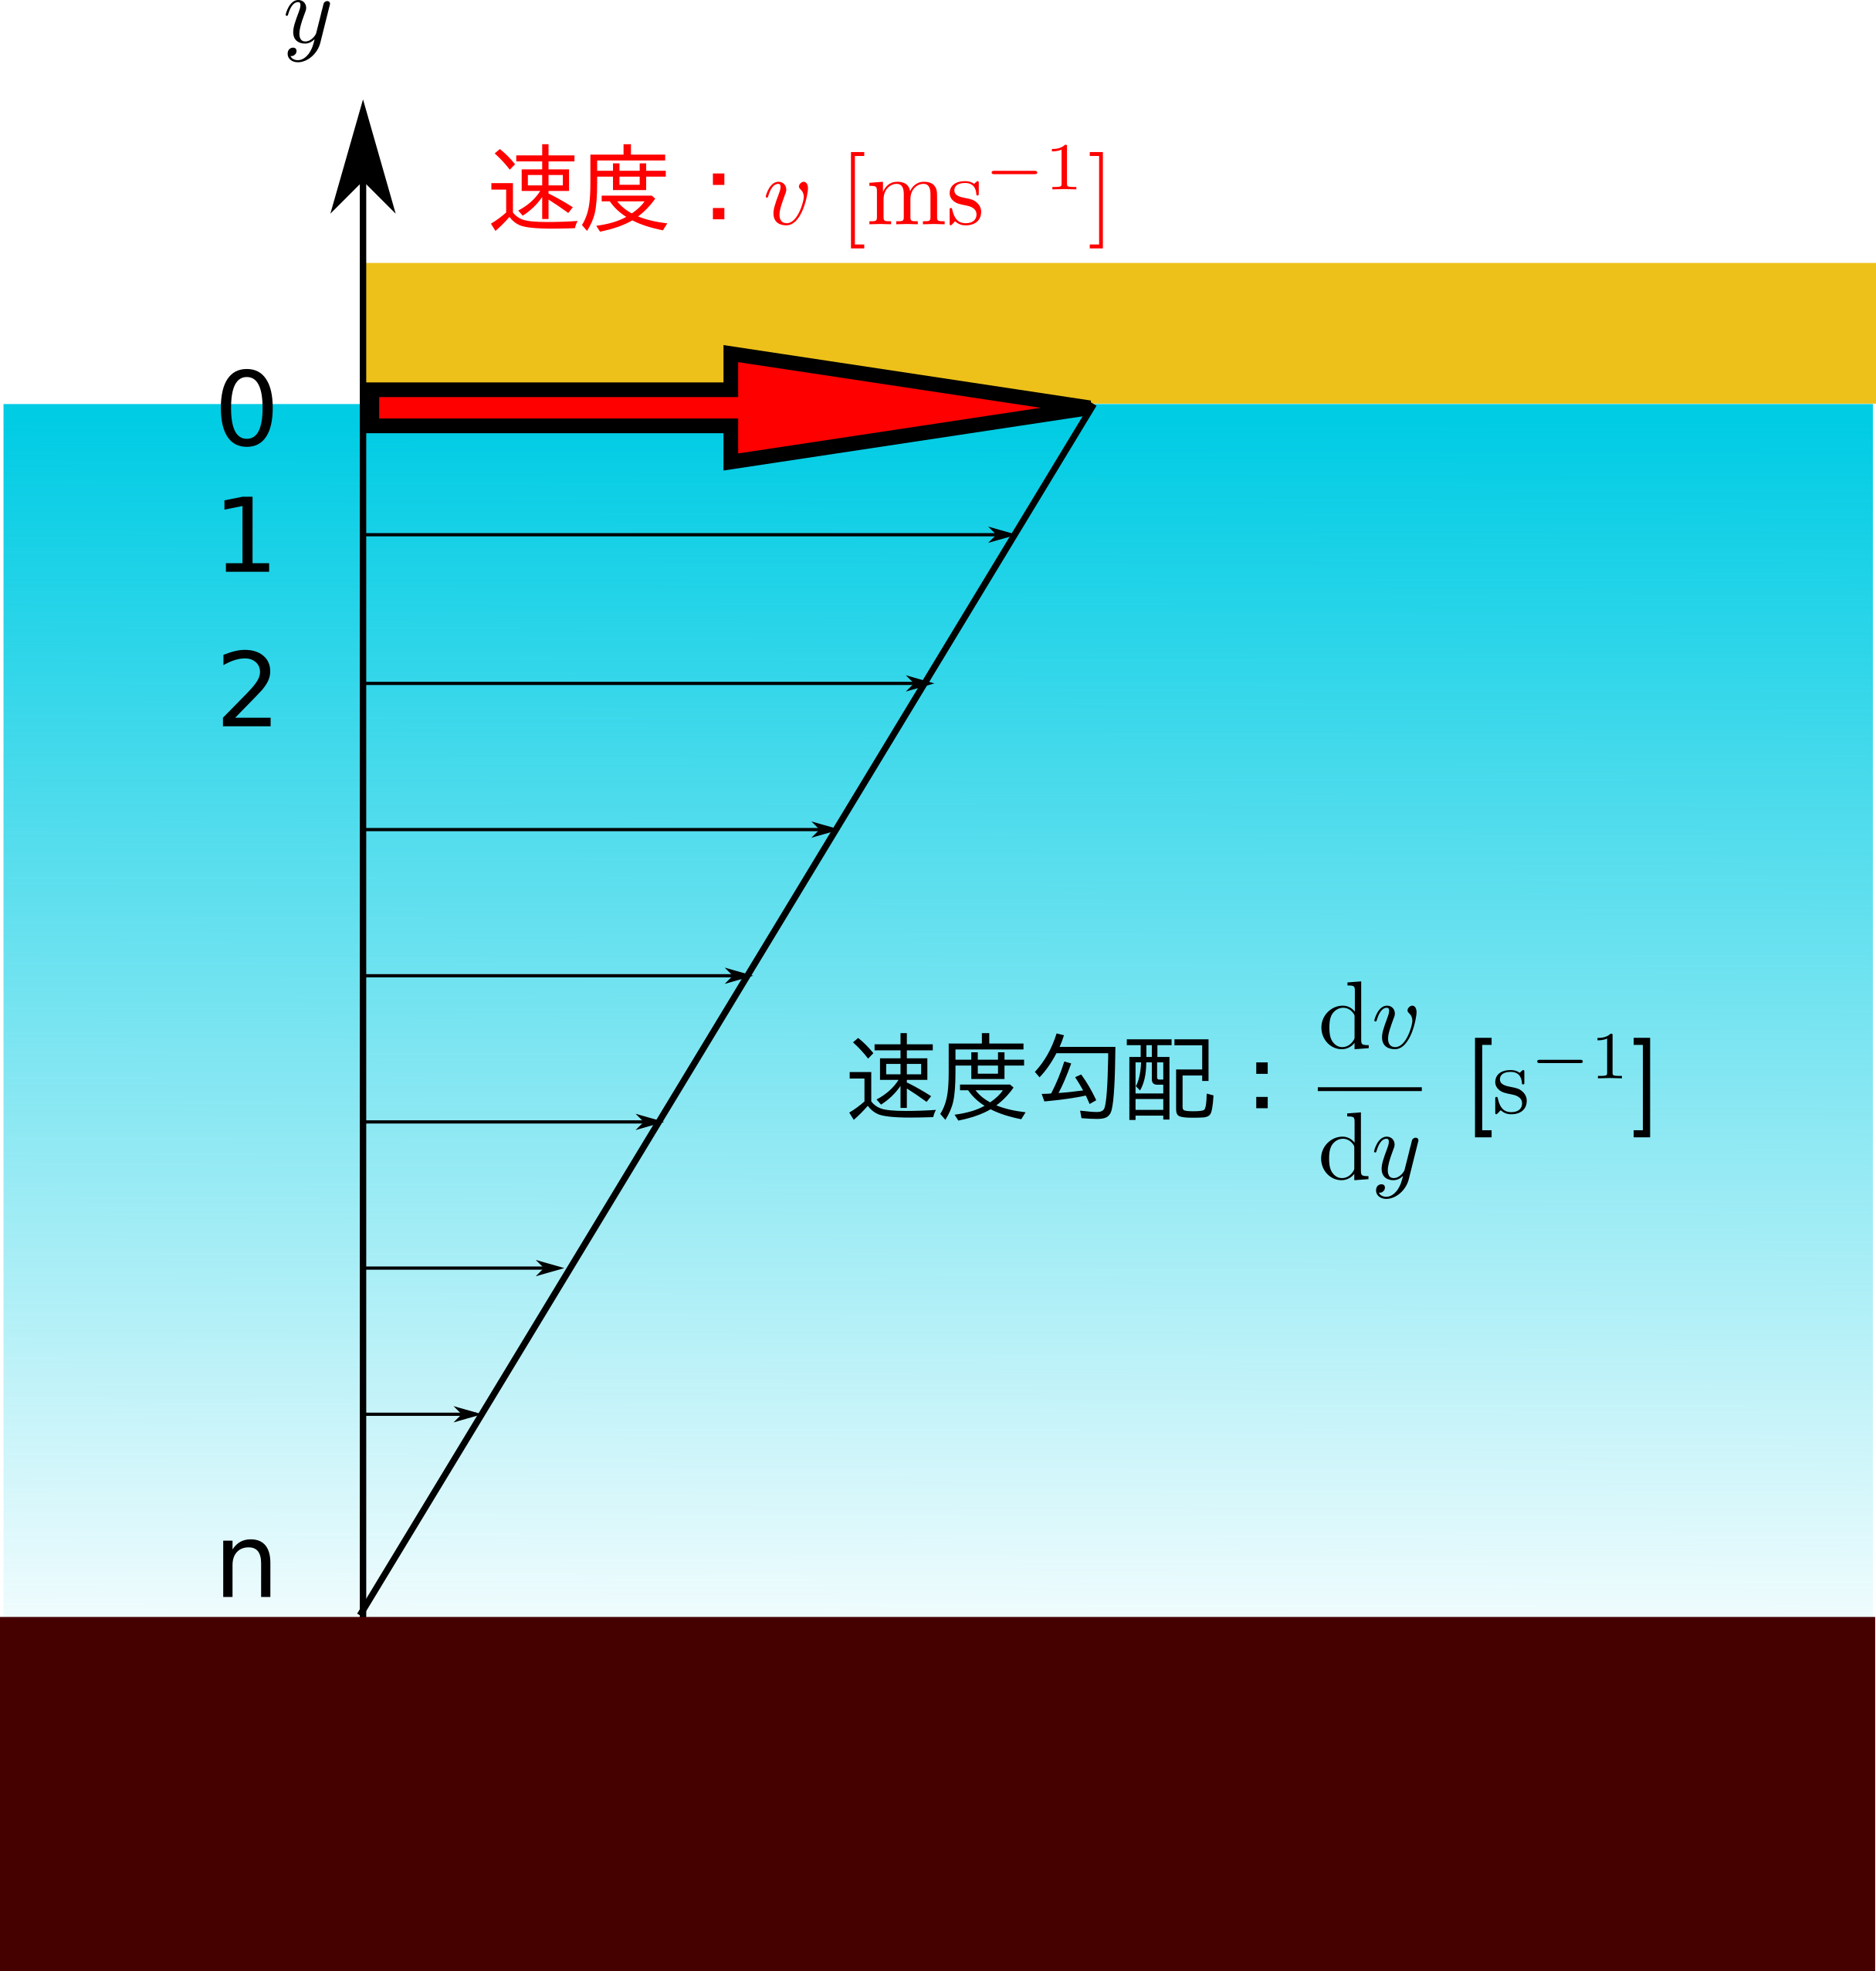
\includegraphics[width=.75\textwidth]{shear_3.png}
					\end{center}
				\end{minipage}
				\begin{minipage}{0.9\textwidth}
					\begin{center}
					\begin{itembox}[l]{注意すべきポイント}
						\begin{itemize}
							\item 固体と接している液体は、その相対的な\qbox{}が同じ。
							\begin{itemize}
								\item 移動する板と接している層 0 は板と同じ速度 $v$ で流れ、
								\item 地面に接している層 $n$ は\qbox{}。
							\end{itemize}
							\item 評価の対象である液体の内部では、
							\begin{itemize}
								\item 水深に応じて、流れる速度の\qbox{}が生じる。
							\end{itemize}
							\item 液体の流れる速度は、
							\begin{itemize}
								\item 水深 $y$ の関数として $v(y)$
								\item \qbox{}と呼ばれ、その単位は $[\mathrm{s^{-1}}]$
							\end{itemize}
						\end{itemize}
					\end{itembox}
					\end{center}
				\end{minipage}
			\end{center}
			
			\vspace{5mm}
			\qitem ニュートン流体について
			\begin{center}
				\begin{minipage}{0.9\textwidth}
					\begin{center}
					\begin{itembox}[l]{ニュートン流体の特徴}
						\begin{itemize}
							\item 「流動を表すモデル」において、速度勾配が\qbox{}となっている。
							\item 速度勾配に従って、各層ごとに\qbox{}が発生
							\begin{itemize}
								\item その値は、局所的なせん断速度に比例して\qbox{}。
								\item 逆に言えば、\qbox{}によらずに\qbox{}が一定。
							\end{itemize}
						\end{itemize}
					\end{itembox}
					\end{center}
				\end{minipage}
			\end{center}

		\end{qlist2}

		\begin{itembox}[l]{選択肢}
			\begin{center}
				\begin{tabular}{lllll}
					1. 分布	&2. せん断応力 &3. 流れない	&4. 速度勾配	&5. 粘度\\
					6. 一定	&7. 変化  &8. せん断速度	&9. 移動速度
				\end{tabular}
			\end{center}
		\end{itembox}
\end{qlist}

\begin{itembox}[l]{解答}
    \begin{center} 
      \begin{tabular}{|c|c|c|c|c|c|c|c|c|c|} \hline
        (a) & (b) & (c) & (d) & (e) & (f) & (g) & (h) & (i)\\ \hline
        9 & 3 & 1 & 8 & 6 & 2 & 7 & 4 & 5 \\ \hline		
      \end{tabular}
    \end{center}
\end{itembox}

\begin{qlist}
	\qitem 「非ニュートン流体」について、\qbox{(j)}から\qbox{(s)}までのカッコを埋めてください。

			\vspace{3mm}
			\begin{qlist2}
			\qitem 非ニュートン流体とは
			\begin{center}
				\begin{minipage}{0.9\textwidth}
					\begin{itembox}[l]{非ニュートン流体とは?}
						\begin{itemize}
							\item 簡単に言えば、ニュートン流動と異なる流動特性を示すものを指します。
							\begin{itemize}
								\item せん断応力が\qbox{}ではない。
								\item 変形状態(せん断速度や加える力が変化)に依存して、\qbox{}が変化する。
							\end{itemize}
							\item その原因は多数あるが、基本的に内部に\qbox{}を有する物質で生じる。
						\end{itemize}
					\end{itembox}
				\end{minipage}

				\vspace{4mm}

				\begin{minipage}{0.43\textwidth}
					\begin{center}
					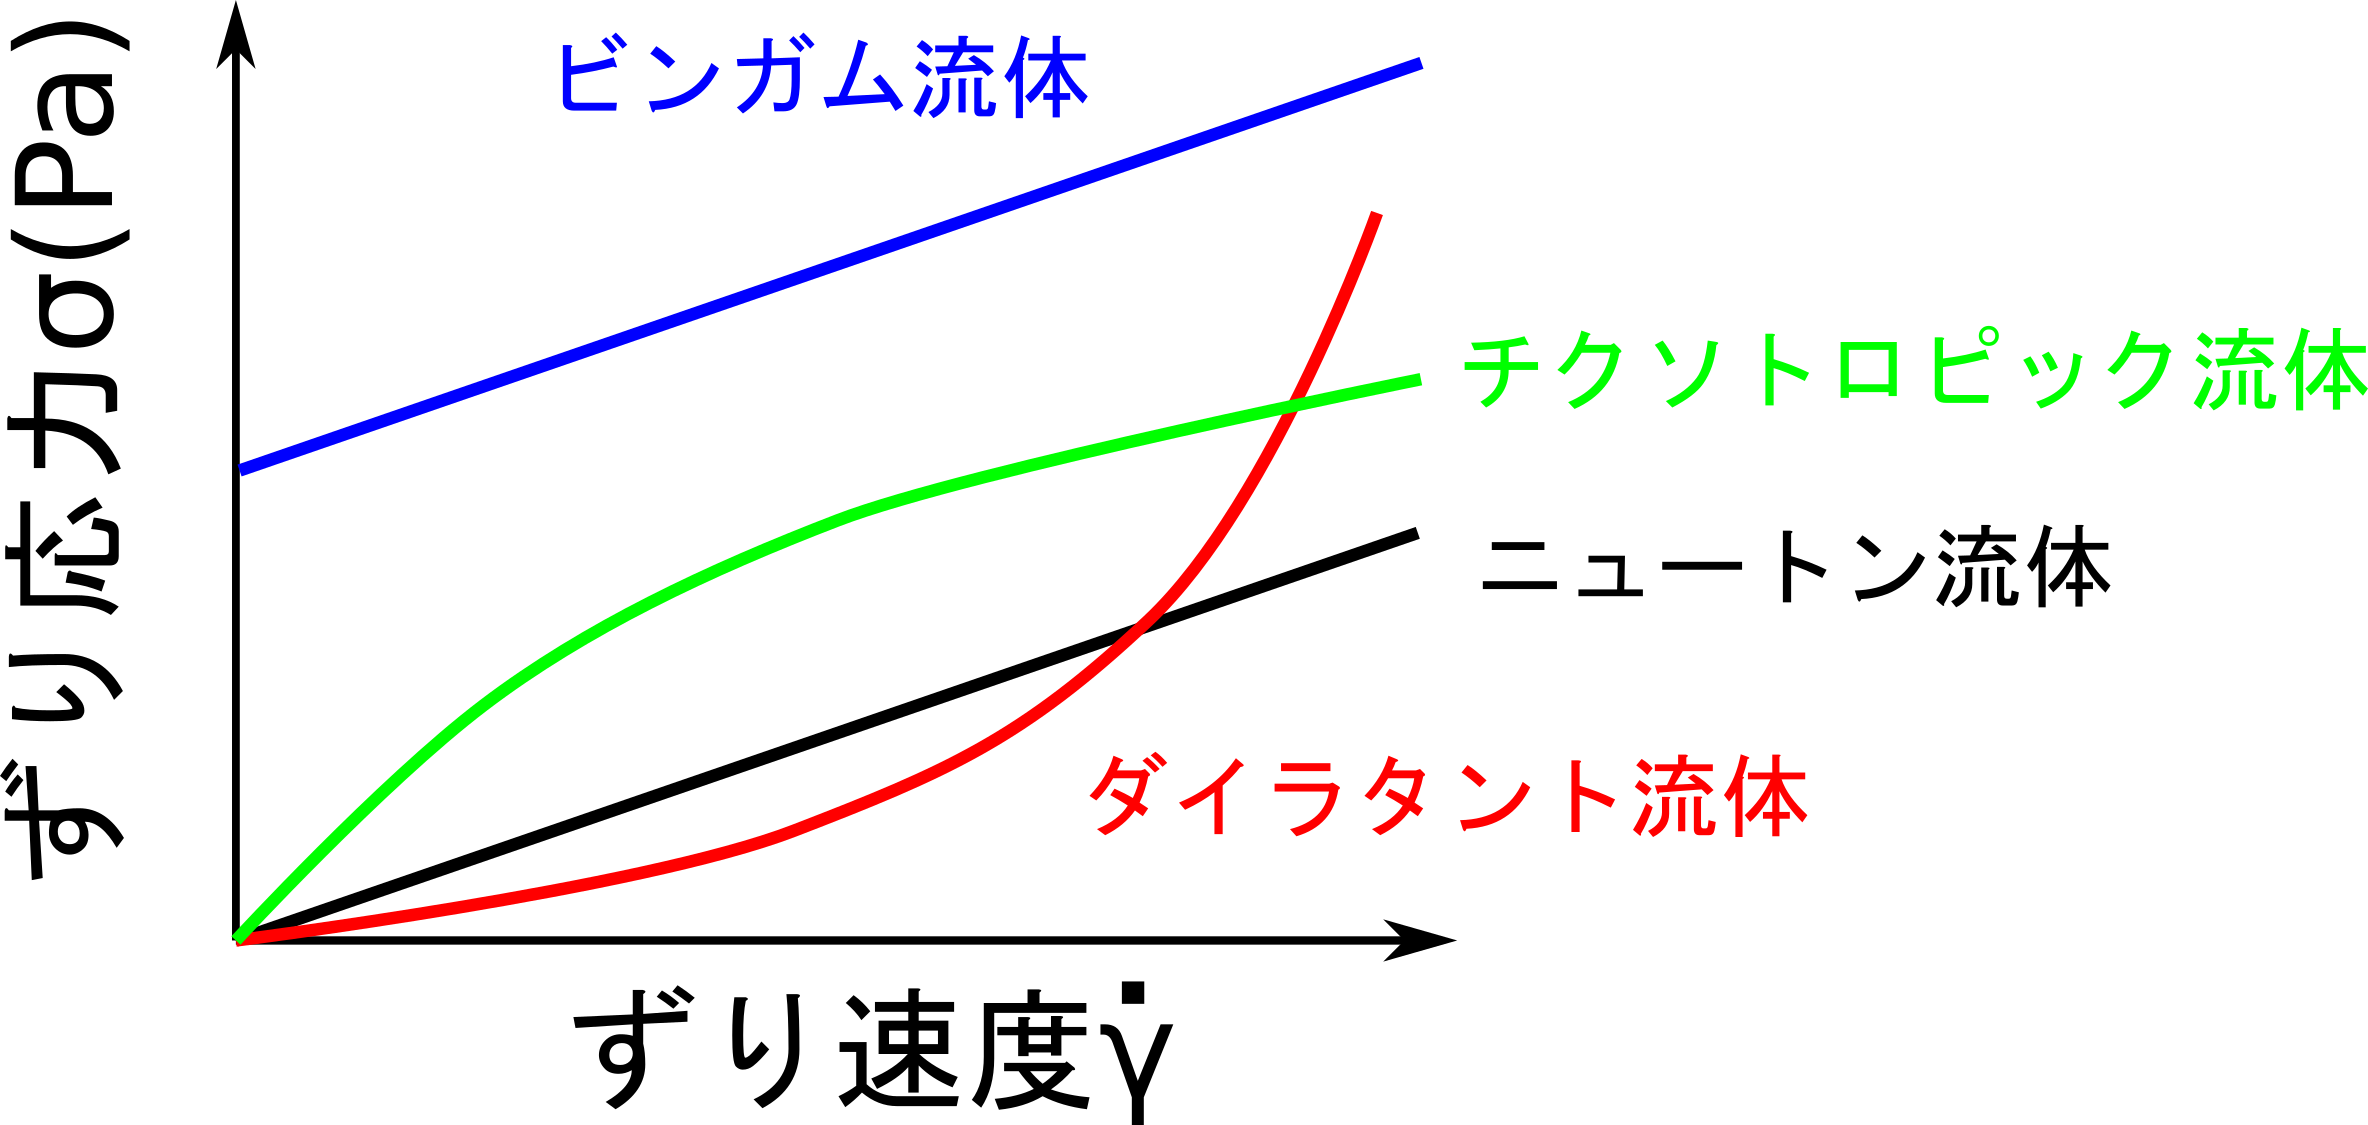
\includegraphics[width=\textwidth]{non_newtonian.png}
					\end{center}
				\end{minipage}
				\begin{minipage}{0.43\textwidth}
					\begin{center}
					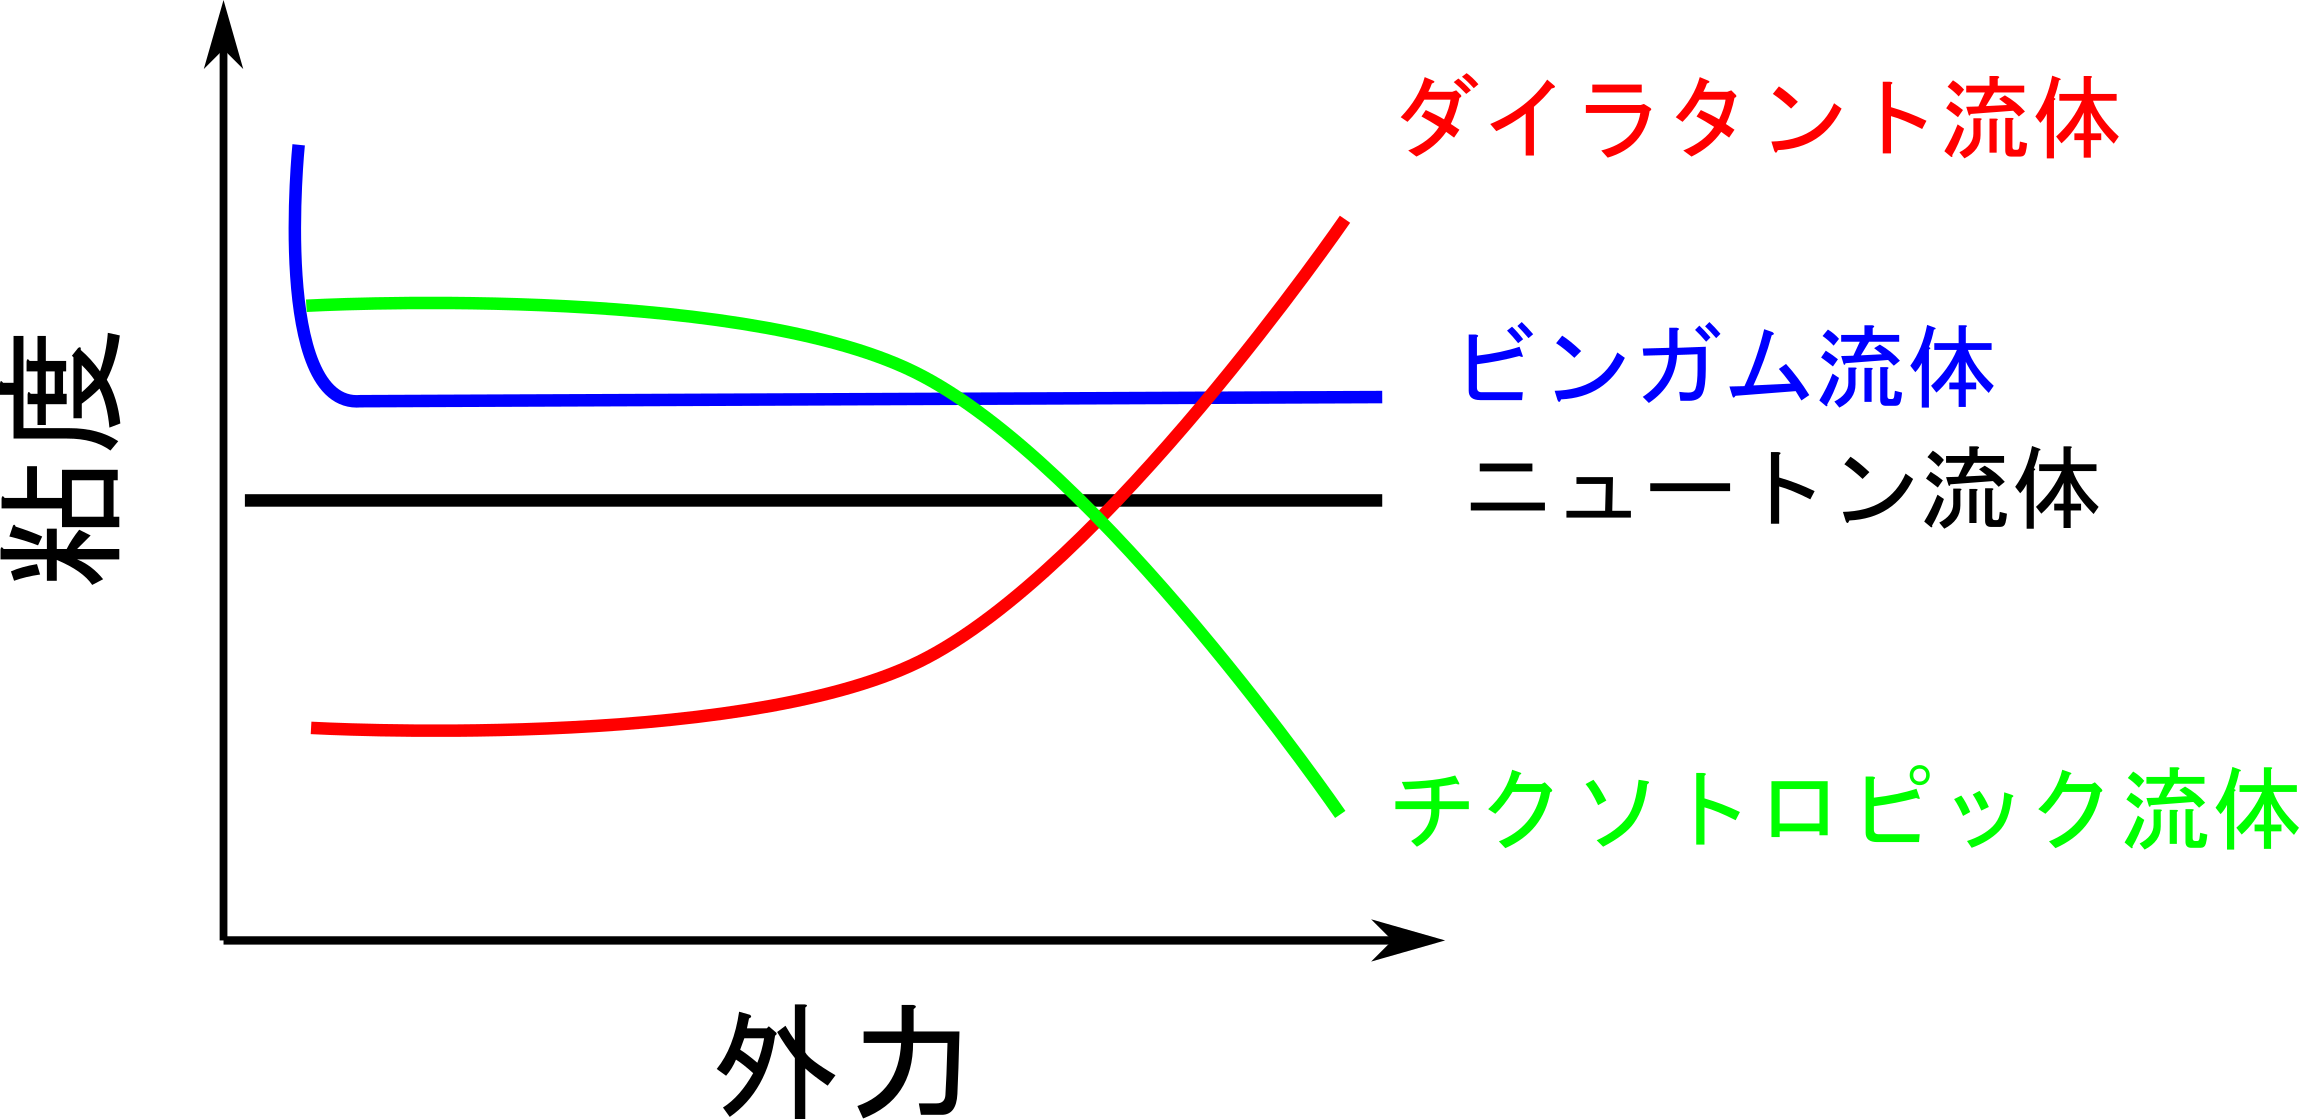
\includegraphics[width=\textwidth]{non_newtonian_2.png}
					\end{center}
				\end{minipage}
			\end{center}

			\vspace{3mm}
			\qitem 非ニュートン流体の発現理由
			\begin{itemize}
				\item 系の挙動を支配する特徴的な時間とは?
				\begin{itemize}
					\item 物質の\qbox{}に由来する特徴的時間が存在し、
					\item これは、内部構造が\qbox{}、再構築するための特徴的な時間と考える。
				\end{itemize}
				\item 外部からの\qbox{}に関わる時間(変形に関与する時間)との関係
				\begin{itemize}
					\item 物質中の内部構造が持つ特徴的な時間よりも短い時間(速い速度)で変形すると、
					\item 内部構造が\qbox{}するため巨視的な粘度が変化し、非ニュートン性が発現する。
				\end{itemize}
			\end{itemize}
			
			\vspace{3mm}
			\qitem シア・シニング(チクソトロピー流体)について
			\begin{center}
				\begin{minipage}{0.5\textwidth}
					\begin{itembox}[l]{シア・シニングの挙動}
						\begin{itemize}
							\item \qbox{}では内部構造が形成されて高粘度。
							\item 高せん断速度が付与されると、
							\begin{itemize}
								\item 内部構造が崩壊し粘度が\qbox{}
							\end{itemize}
							\item せん断速度の低下により粘度が、\qbox{}。
						\end{itemize}
					\end{itembox}
				\end{minipage}
				\begin{minipage}{0.38\textwidth}
					\begin{center}
					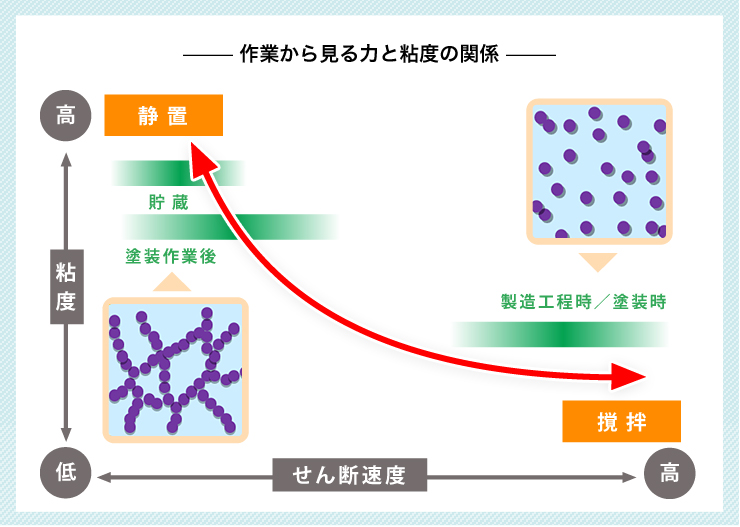
\includegraphics[width=1.2\textwidth]{thixotropy_1w.jpg}
					\end{center}
				\end{minipage}
			\end{center}

		\end{qlist2}

		\begin{itembox}[l]{選択肢}
			\begin{center}
				\begin{tabular}{lllll}
					1. 内部構造	&2. 粘度	&3. 構造	&4. 低下 &5. 再上昇\\
					6. 静置状態	&7. 崩壊	&8. 変形	&9. 線形 &10. 変化
				\end{tabular}
			\end{center}
		\end{itembox}
\end{qlist}

\begin{itembox}[l]{解答}
    \begin{center} 
      \begin{tabular}{|c|c|c|c|c|c|c|c|c|c|} \hline
        (j) & (k) & (l) & (m) & (n) & (o) & (p) & (q) & (r) & (s)\\ \hline
        9 & 2 & 3 & 1 & 10 & 8 & 7 & 6 & 4 & 5 \\ \hline		
      \end{tabular}
    \end{center}
\end{itembox}

\question{演習問題 3}
説明文中の言葉を使って数行程度の簡単な記述で構いませんので、以下の自由記述問題を考えてみてください。
\begin{qlist}
\qitem この章では、実際の我々の身の回りにある少しだけ複雑な事象についての説明を行うために、
まず、最もシンプルなニュートン流体の流動を表すモデルを振り返りました。
そして、非ニュートン流体という複雑な流れ方がなぜ生じるのかということを、ニュートン流動との相違という形で説明しました。

ご自身の興味のある非ニュートン流動について、文中の言葉をそのまま使って結構ですから、簡単に書いてみてください。
\end{qlist}

\begin{itembox}[l]{解答例}
    私は、この議論では余り詳細に立ち入っていないシア・シックニングに興味を持っています。
	一般に、ダイラタンシーと呼ばれる現象です。

	この現象は、別に、水の上を走って渡れるというようなお遊び的なものだけではなく、普段は柔軟で衝撃を付与したときだけ衝撃吸収しながら防御できる防弾チョッキのような応用も提案されています。
	このような新規機能を設計できたらと望んでいます。	
\end{itembox}

\clearpage

\end{document}